\section{CIG: Computational\\ Intelligence in Games}\label{subsecCIG}

% co-exists with CIG conference
% games are run privately on several computers just before the conference  
The CIG StarCraft RTS AI Competition is a part of the program of the IEEE Computational Intelligence in Games (CIG) conference since August 2010. Similarly to AIIDE competition, all the bot games are run separately on several computers prior to the conference and the results are then announced during the event. Unlike in AIIDE and SSCAIT, the map pool of the CIG competition is not known in advance for the competitors. Also, the CIG competition no longer enforces an open source code requirement to compete.

\subsection*{CIG 2016-17 Updates \& News}\label{subsecCIGnews}

% CIG 2017 scheduled for Summer 2017
% CIG 2016 happened in Sept. 2016.  
CIG 2017 is scheduled to happen in New York City, USA on late August 2017, which is just after the submission deadline of this paper. Therefore, we will report on CIG 2016, which happened on September 2016. 

% two round-robin stages: qualifying stage and final stage. half of Q goes to F
% persistent files are erased between stages 
% qualif. stage: 11988 games with 16 bots
% final stage: 2799 games with 8 bots
% ran for 8 days on 17 computers
% winner: tscmoo by Vegard Mella from Norway

The 2016 installment of CIG competition hosted {\em 16 participants}, out of which 9 were new or updated bots and 7 were re-entries from previous year. CIG 2016 competition was divided into two stages: The {\em Qualifying} stage and the {\em Final} stage. The first qualifying stage consisted of Round Robin tournament between all 16 participating bots. In total, 11988 games were played in this stage. After the qualifying stage, best 8 bots were selected to proceed to the final stage: {\em tscmoo, IronBot, LetaBot, ZZZbot, Overkill, UAlbertaBot, MegaBot} and {\em Aiur}.

All the persistent files accumulated by the bots in the qualifying stage were deleted before entering the finals. This stage consisted of 2799 Round Robin games between the 8 bots. All the games ran on 17 computers for 8 days. The winner of the final stage, {\em tscmoo} bot created by Vegard Mella from Norway, was announced the overall winner of CIG 2016 tournament with 456 wins and $65.14\%$ win rate in the final stage. Detailed results are depicted in Figure~\ref{figCIGresults}. 

\begin{figure}[h]
  \centering
  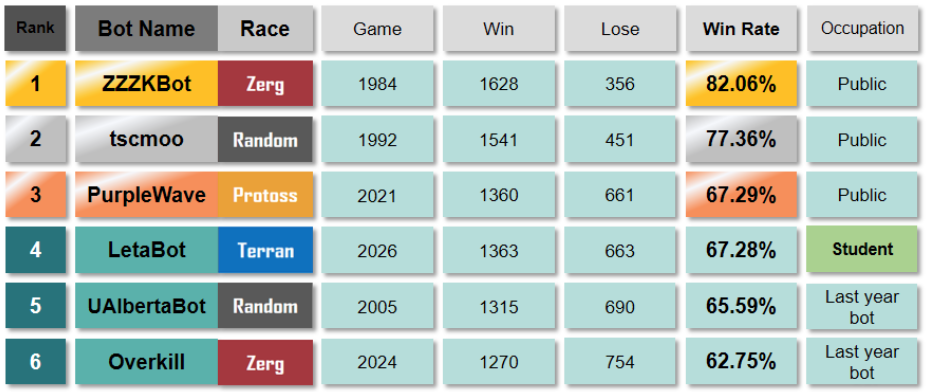
\includegraphics[width=0.5\textwidth]{fig/cig-results.png}
  \caption{Detailed results of the CIG 2016 competition final stage.}
  \label{figCIGresults}
\end{figure}
